\chapter{Programación Paralela}

En el capítulo anterior, nos dedicamos a introducir los conceptos de paralelismo dentro de una aplicación, tanto a nivel implícito como explícito; así como formas de llevarlo a cabo y de evaluación de las mejoras relacionadas con implementar paralelismo. A continuación, nos toca conocer a un menor nivel de abstracción cómo se programan todas estas estrategias relacionadas con el paralelismo que ya hemos desarrollado y que el lector debería comprender.

\section{Estructuras en programación paralela}
En esta sección, planteamos los aspectos particulares de las herramientas de programación paralela (aquellas que nos ayudan a desarrollar código paralelo, para poder crear aplicaciones paralelas). Haremos incapié en el trabajo extra que supone hacer una aplicación paralela frente a una secuencial, así como aprender formas de comunicación (o sincronización) que se ofertan al programador.

\subsection{Objetivos}
En esta sección, tratamos de:
\begin{itemize}
    \item Distinguir entre los diferentes tipos de herramientas de programación paralela, como compiladores paralelos, lenguajes paralelos, APIs de directivas y APIs de funciones.
    \item Distinguir entre los diferenties tipos de comunicaciones colectivas.
    \item Diferenciar el paradigma de programación de paso de mensajes con respecto al paradigma de variables compartidas.
    \item Diferenciar entre OpenMP y MPI, en cuanto a su estilo de programación y tipo de herramienta.
    \item Distinguir entre las esctructuras de tareas junto a procesos y hebras, master-slave, cliente-servidor, descomposición de dominio, flujo de datos (o segmentación) y divide y vencerás.
\end{itemize}

\subsection{Problemas que plantea la programación paralela}
La programación paralela requiere de algún ente (ya sea la herramienta que usemos o el propio programador) que realice el trabajo necesario para llevar a cabo el paralelismo, a diferencia de un código secuencial. Los mayores trabajos (y los más comunes) que nos encontramos a la hora de pasar de una aplicación secuencial a una paralela los desarrollaremos a continuación.

\begin{description}
    \item [Localicación o detección de paralelismo]~\\
        Para poder implementar paralelismo dentro de una aplicación, esto es, dividir las aplicaciones en unidades de cómputo independientes que recibirán el nombre de \emph{tareas}, es necesario primero localizar de dónde podemos extraer este paralelismo. Lo más cómodo y usual será, a partir del código secuencial que resuelve nuestra aplicación (o a partir de la definición de la aplicación), analizarlo para ver de dónde podemos extraer paralelismo (y en qué parte del código es donde debemos intentar introducir paralelismo). Los grafos pueden ser una gran herramienta en esta tarea, ya que nos permiten ver las tareas que pueden ejecutarse en paralelo (estos serán los nodos a misma altura, si la altura representa el tiempo de ejecución); así como las dependencias que hay entre ellas (los datos que una tarea requiere de otra para su ejecución). Finalmente, también nos permite ver cuál es el número máximo de tareas que se ejecutarán en paralelo. A este número máximo se le suele llamar \emph{grado de paralelismo} de una aplicación.
    \item [Asignación de carga de trabajo]~\\
        Tenemos que decidir qué tareas corresponderán a qué ente del sistema operativo (como procesos o \emph{threads}), así como la asignación de flujos de instrucciones\footnote{Cada vez que mencionemos este concepto, nos estaremos refierendo a procesos o hilos (entes del sistema operativo).} a los procesadores disponibles. Cabe destacar que no suele ser rentable usar más flujos de instrucciones que procesadores ni que los flujos cambien de procesador en tiempo de ejecución. Así, las asignaciones de flujos a procesadores puede hacerse estática o dinámicamente (en tiempo de ejecución); y de forma explícita o implícita (lo hace la herramienta de forma automática). Notemos que la asignación dinámica requiere un costo extra, lo que introduce un retardo adicional. La asignación dinámica es la única posible cuando no puede conocerse el número de tareas a ejecutar. 
    \item [Comunicación o sincronización]~\\
        Muchas veces necesitaremos mecanismos de comunicación entre los distintos flujos de instrucciones, ya que todos estos están colaborando en la ejecución del programa (uno puede generar una variable que otro necesite). 
\end{description}

Un ejemplo de la necesidad de todas estas tareas la vemos reflejada en el siguiente código:
    \begin{minted}[xleftmargin=1cm]{c++}
main(int argc, char** argv){
    double ancho, sum = 0;
    int intervalos, i;
    
    intervalos = atoi(argv[1]);
    ancho = 1.0/(double) intervalos;

    for(int i = 0; i < intervalos; i++){
        x = (i+0.5) * ancho;
        sum += 4.0/(1.0 + x * x);
    }

    sum *= ancho;
    // ...
}
    \end{minted}
\label{codigo_pi}
Tenemos un código secuencial que se encarga de realizar una tarea determinada. Ahora, queremos hacer uso del paralelismo para disminunir el tiempo de ejecución de la tarea. Vemos cómo hacerlo en la siguiente figura, donde hemos hecho uso de la herramienta OpenMP.
    \begin{minted}[xleftmargin=1cm]{c++}
#include <omp.h>
#define NUM_THREADS 4

main(int argc, char** argv){
    double ancho, sum = 0;
    int intervalos, i;
    
    intervalos = atoi(argv[1]);
    ancho = 1.0/(double) intervalos;
    omp_set_num_threads(NUM_THREADS);

    #pragma omp parallel for reduction(+:sum) private(x)
    for(int i = 0; i < intervalos; i++){
        x = (i+0.5) * ancho;
        sum += 4.0/(1.0 + x * x);
    }

    sum *= ancho;
    // ...
}
    \end{minted}
En primer lugar, hemos detectado qué parte podríamos mejorar del código. En este caso, repartir las iteraciones del bucle entre distintas hebras, ya que las iteraciones no están relacionadas entre sí. A continuación, hemos decidido que vamos a usar 4 hebras, y que vamos a repartir las \verb|intervalos| iteraciones de forma equitativa entre las 4 hebras. Finalmente, comunicamos las hebras entre sí gracias a dos palabras:
\begin{itemize}
    \item La cláusula \verb|reduction(+:sum)| nos permite sumar en \verb|sum| los distintos valores de la variable \verb|sum| de cada hebra (cabe destacar que lo podríamos haber hecho con un proceso menos automático y más personalizado, como con la directiva \verb|critical|, aunque en este caso la mejor elección es \verb|atomic| debido a la simplicidad de la comunicación a realizar).
    \item La directiva \verb|for| tiene una barrera implícita al final que hace que todas las hebras se esperen entre sí (tarea de sincronización).
\end{itemize}

\subsubsection{Modos de programación}
A la hora de programar una aplicación paralela, podemos distinguir dos modos de programación:
\begin{description}
    \item [SPMD (\emph{Single-Program Multiple Data})]~\\
        También denominado a veces paralelismo de datos, todos los códigos que se ejecutan en paralelo se obtienen compilando el mismo programa. Cada copia trabaja con un conjunto de datos distinto y se ejecuta en un procesador diferente.
    \item [MPMD (\emph{Multiple-Program Multiple Data})]~\\
        También llamado a veces paralelismo de tareas o funciones, los códigos que se ejecutan en paralelo se obtienen compilando programas independientes. En este caso, la aplicación a ejecutar (o el código secuencial inicial) se divide en unidades independientes. Cada unidad trabaja con un conjunto de datos distintos y se ejecutan en un procesador diferente.
\end{description}

SPMD es recomendable en sistemas masivamente paralelos. Es más fácil resolver la aplicación escribiendo un único programa. Usado en sistemas con memoria distribuida, evita la necesidad de tener que distribuir el código entre los nodos, solo habría que distribuir datos. En la práctica, se aplica en mayor medida SPMD antes que MPMD.

En los programas paralelos se pueden utilizar combinaciones de MPMD y SPMD\@. La programación dueño-esclavo se puede considerar una variante del modo MPMD (se verá a lo largo de esta sección). Si todos los esclavos tienen el mismo código, sería una mezcla de MPMD y SPMD\@. Los programas que conforman una solución dueño-esclavo con MPMD se pueden juntar en un único programa SPMD con el uso de estructuras condicionales.

\subsection{Herramientas para obtener código paralelo}
Las herramientas de programación paralela debería permitirnos de forma explícita o implícita:
\begin{enumerate}
    \item Localizar paralelismo: descomponer la aplicación en tareas independientes.
    \item Asignar las tareas: repartir la carga de trabajo entre procesos.
    \item Crear (enrolar) y terminar (desenrolar) procesos.
    \item Comunicar y sincronizar procesos.
    \item Asignar procesos a procesadores.
\end{enumerate}
Respecto a este último aspecto, es el SO o el hardware quien se encarga (usualmente) de ello.\\

Cuanto mayor sea la abstracción que desarrolle la herramienta paralela, menor serán las labores que debe desarrollar el programador de aplicaciones paralelas. La labor más difícil para la herramienta es la primera, la detección del paralelismo. Podemos realizar una clasificación de las herramientas de programación paralela en función de la abstracción en la que sitúan al programador. Las enumeramos desde el mayor al menor nivel de abstracción:
\begin{description}
    \item [Compiladores paralelos]~\\
        Un compilador paralelo pretende ser aquella automatización capaz de extraer paralelismo a nivel de bucle (paralelismo de datos) y de función (paralelismo de tareas) a partir de un código secuencial. Para ello, realizan análisis de dependencias entre bloques de código. No generan código eficiente para cualquier programa y todavía se investiga en este campo.
    \item [Lenguajes paralelos y APIs de funciones y directivas]~\\
        Generalmente, los lenguajes paralelos y APIs de directivas sitúan al programador en un nivel de abstracción superior al proporionado solo por bibliotecas de funciones. Encontramos lenguajes como Occam, Ada o Java, los cuales tienen construcciones particulares y bibliotecas de funciones que requieren un compilador exclusivo. Por otra parte, las APIs mencionadas (formadas tanto por directivas para el lenguaje como por bibliotecas de funciones) nos permiten trabajar en cualquier lenguaje para el que fueron diseñadas, como C\verb|++| o Fortran, en el caso de OpenMP\@. En este nivel, el programador es el encargado de detectar el paralelismo implícito en la aplicación. Sin embargo, el programador no hace el reparto (la asignación directa) de este paralelismo, así de eximir al programador las tareas de creación y terminación de flujos o de detalles para comunicación. Como ventaja, es más sencillo desarrollar aplicaciones paralelas, obteniendo códigos más cortos.
    \item [APIs de funciones]~\\
        Como por ejemplo Pthreads o MPI, las cuales solo consisten en una biblioteca de funciones que se añaden a un compilador de un lenguaje sencuencial. El cuerpo de procesos y hebras es escrito en lenguaje secuencial y es el programador quien se encarga de distribuir las tareas entre los procesos, crear o gestionar procesos, e implementar la comunicación y sincronización usando funciones de la biblioteca. Como ventajas a destacar:
        \begin{itemize}
            \item Los programadores están familiarizados con los lenguajes secuenciales.
            \item Las bibliotecas están disponibles para todos los sistemas paralelos.
            \item Las bibliotecas están más cercanas al hardware y permiten dar al programador un control a más bajo nivel.
            \item Se pueden utilizar a la vez bibliotecas para programar con hebras y con procesos.
        \end{itemize}
    \item [Lenguajes paralelos para arquitecturas de propósito específico]~\\
        Como por ejemplo CUDA (de NVIDIA). Consisten en construcciones del lenguaje y bibliotecas de funciones que requieren un compilador exclusivo. El programador debe participar en todas las labores salvo quizás en la asignación de flujos de instrucciones a unidades de procesamiento. Debe tener un gran conocimiento de las arquitecturas para poder escribr el código paralelo.
\end{description}

Comentamos ahora que, mientras OpenMP es el estándar industrial en programación paralela (gracias al alto nivel de abstracción que provee al programador), MPI es el estándar industrial para la programación de multicomputadores. OpenMP realiza de forma automática el reparto de trabajo, mientras que en MPI es el programador quien debe llevarlo a cabo (esto es lógico, debido al estar orientado a multicomputadores, donde el reparto de la carga de trabajo es más difícil de realizar, como ya vimos en el capítulo anterior).

\subsection{Comunicaciones y sincronizaciones}
Las herramientas para la programación paralela también pueden ofrecer al programador, además de la comunicación entre dos procesos, comunicaciones en las que intervienen múltiples procesos. Estas comunicaciones se implementan para comunicar a todos los procesos que forman parte del grupo que colabora en la ejecución de un código. En muchos casos estas comunicaciones no tienen la finalidad de transmitir datos, sino de sincronizar procesos. Es común ver en varias aplicaciones las funcionalidades de:
\begin{itemize}
    \item Reordenar datos entre procesos.
    \item Difusión de datos.
    \item Reducir un conjunto de datos a uno solo.
    \item Múltiples reducciones en paralelo con el mismo conjunto de datos.
    \item Sincronizar múltiples procesos en un punto.
\end{itemize}

Por tanto, se intenta que las herramientas de programación paralela nos permitan implementar dichas funcionalidades mediante comunicaciones entre procesos (flujos de instrucciones). A lo largo de esta sección, cada vez que aparezca ``mensaje'', estaremos haciendo referencia a un dato o estructura de datos. A continuación, enumeramos los distintos tipos de comunicaciones entre procesos que podemos encontrarnos:
\begin{description} 
    \item [Comunicación múltiple uno-a-uno] Hay componentes del grupo que envían un único mensaje y componentes que reciben un único mensaje. Si todos los componentes del grupo envían y reciben, diremos que se trata de una \emph{permutación}. Nos podemos encontrar \emph{rotaciones} (el proceso $P_i$ envía al proceso $P_{i+1}$ y el $P_n$ al $P_0$), \emph{intercambios}, \emph{barajes}, \emph{desplazamientos}, etc. (Ver Figura~\ref{graph:uno_uno}).

    \item [Comunicación uno-a-todos] Un proceso envía y todos los procesos del grupo reciben el mensaje (Ver Figura~\ref{graph:uno_todos}). Destacamos aquí:
        \begin{description}
            \item [Difusión (broadcast)] Todos los procesos reciben el mismo mensaje.
            \item [Dispersión (scatter)] Cada proceso recibe un mensaje diferente.
        \end{description}

    \item [Comunicación todos-a-uno] Todos los procesos en el grupo envían un mensaje a un único proceso (Ver Figura~\ref{graph:todos_uno}). Destacamos:
        \begin{description}
            \item [Reducción] Los mensajes enviados por los procesos se combinan en un solo mensaje mediante algún operador (como por ejemplo, el proceso recibe una suma de distintas variables de cada proceso).
            \item [Acumulación (gather)] Los mensajes se reciben de forma concatenada en el receptor.
        \end{description}

    \item [Comunicación todos-a-todos] Todos los procesos del grupo ejecutan una comunicación uno-a-todos (Ver Figura~\ref{graph:todos_todos}). Puede ser:
        \begin{description}
            \item [Todos difunden (all-broadcast)] Todos los procesos realizan una difusión.
            \item [Todos dispersan (all-scatter)] Todos los procesos realizan una dispersión.
        \end{description}

    \item [Comunicaciones colectivas compuestas] Hay servicios que resultan de la combinación de algunos anteriores, como:
        \begin{description}
            \item [Todos combinan, o reducción y extensión] El resultado de aplicar una reducción se obtiene en todos los procesos (Ver Figura~\ref{graph:colectivas1}).
            \item [Barrera] Es un punto de sincronización que todos los procesos de un grupo deben alcanzar para que cualquier proceso del grupo pueda continuar con su ejecución.
            \item [Recorrido (scan)] Todos los procesos envían un mensaje, recibiendo cada uno de ellos el resultado de reducir un conjunto de estos mensajes (Ver Figura~\ref{graph:colectivas2}).
                \begin{itemize}
                    \item Recorrido prefijo: El proceso $P_i$ recibe el resultado de reducir los mensajes de $P_0, P_1, \ldots, P_i$.
                    \item Recorrido sufijo: El proceso $P_i$ recibe el resultado de reducir los mensajes de $P_i, P_{i+1}, \ldots, P_n$.
                \end{itemize}
        \end{description}
\end{description}

Comunicaciones como ``dispersión'' o ``todos dispersan'' son usadas para reparto de datos. ``Acumulación'' es usada para fusionar datos intermedios. Los ``desplazamientos'' son tramos intermedios para realizar nuevos repartos de datos.\\

% ----------------------------------------------------------------------

\begin{figure}
\centering
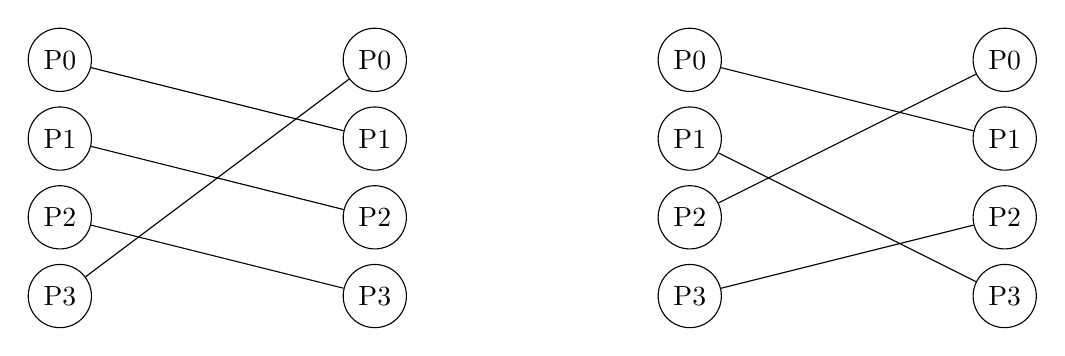
\begin{tikzpicture}
  % Nodos
    % Rotacion
    \node[draw, circle] (A) at (0,3) {P0};
    \node[draw, circle] (B) at (0,2) {P1};
    \node[draw, circle] (C) at (0,1) {P2};
    \node[draw, circle] (D) at (0,0) {P3};
    \node[draw, circle] (E) at (4,3) {P0};
    \node[draw, circle] (F) at (4,2) {P1};
    \node[draw, circle] (G) at (4,1) {P2};
    \node[draw, circle] (H) at (4,0) {P3};

    % Permutacion
    \node[draw, circle] (I) at (8,3) {P0};
    \node[draw, circle] (J) at (8,2) {P1};
    \node[draw, circle] (K) at (8,1) {P2};
    \node[draw, circle] (L) at (8,0) {P3};
    \node[draw, circle] (M) at (12,3) {P0};
    \node[draw, circle] (N) at (12,2) {P1};
    \node[draw, circle] (O) at (12,1) {P2};
    \node[draw, circle] (P) at (12,0) {P3};

  % Aristas
    % Rotacion
    \draw (A) -- (F);
    \draw (B) -- (G);
    \draw (C) -- (H);
    \draw (D) -- (E);

    % Permutacion
    \draw (I) -- (N);
    \draw (K) -- (M);
    \draw (J) -- (P);
    \draw (L) -- (O);
\end{tikzpicture}
\caption{Dos permutaciones, la primera de ellas rotación.}
\label{graph:uno_uno}
\end{figure}

\begin{figure}
\centering 
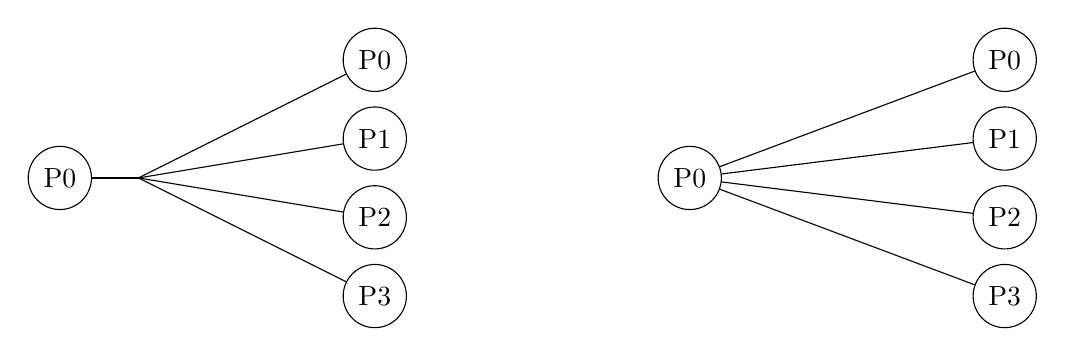
\begin{tikzpicture}
    % Nodos
    % Difusion
    \node[draw, circle] (A) at (0,1.5) {P0};
    \node[draw, circle] (B) at (4,0) {P3};
    \node[draw, circle] (C) at (4,1) {P2};
    \node[draw, circle] (D) at (4,2) {P1};
    \node[draw, circle] (E) at (4,3) {P0};

    % Dispersion
    \node[draw, circle] (F) at (8,1.5) {P0};
    \node[draw, circle] (G) at (12,0) {P3};
    \node[draw, circle] (H) at (12,1) {P2};
    \node[draw, circle] (I) at (12,2) {P1};
    \node[draw, circle] (J) at (12,3) {P0};

    % Nodos
    % Difusion
    \draw (A) -- (1, 1.5);
    \draw (1, 1.5) -- (B);
    \draw (1, 1.5) -- (C);
    \draw (1, 1.5) -- (D);
    \draw (1, 1.5) -- (E);

    % Dispersion
    \draw (F) -- (G);
    \draw (F) -- (H);
    \draw (F) -- (I);
    \draw (F) -- (J);
\end{tikzpicture}
\caption{Una difusión a la izquierda y una dispersión a la derecha.}
\label{graph:uno_todos}
\end{figure}

\begin{figure}
\centering 
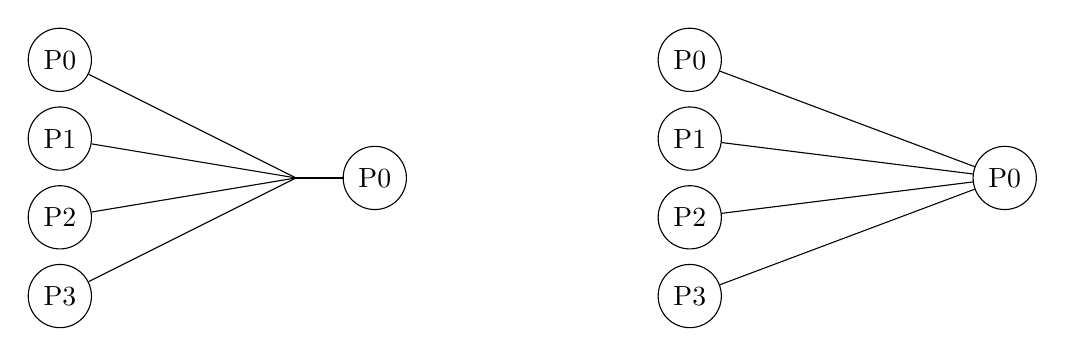
\begin{tikzpicture}
    % Nodos
    % Difusion
    \node[draw, circle] (A) at (4,1.5) {P0};
    \node[draw, circle] (B) at (0,0) {P3};
    \node[draw, circle] (C) at (0,1) {P2};
    \node[draw, circle] (D) at (0,2) {P1};
    \node[draw, circle] (E) at (0,3) {P0};

    % Dispersion
    \node[draw, circle] (F) at (12,1.5) {P0};
    \node[draw, circle] (G) at (8,0) {P3};
    \node[draw, circle] (H) at (8,1) {P2};
    \node[draw, circle] (I) at (8,2) {P1};
    \node[draw, circle] (J) at (8,3) {P0};

    % Nodos
    % Difusion
    \draw (A) -- (3, 1.5);
    \draw (3, 1.5) -- (B);
    \draw (3, 1.5) -- (C);
    \draw (3, 1.5) -- (D);
    \draw (3, 1.5) -- (E);

    % Dispersion
    \draw (F) -- (G);
    \draw (F) -- (H);
    \draw (F) -- (I);
    \draw (F) -- (J);
\end{tikzpicture}
\caption{Una reducción a la izquierda y una acumulación a la derecha.}
\label{graph:todos_uno}
\end{figure}

\begin{figure}
\centering 
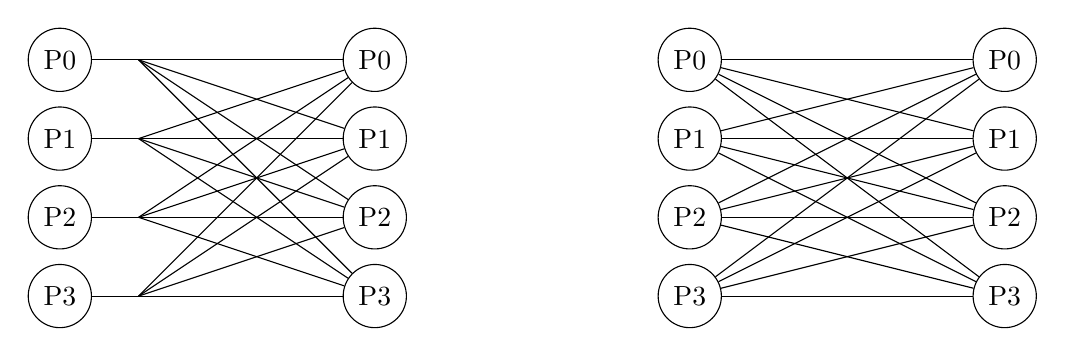
\begin{tikzpicture}
    % Nodos de todos difunden
    \node[draw, circle] (A) at (0,3) {P0};
    \node[draw, circle] (B) at (0,2) {P1};
    \node[draw, circle] (C) at (0,1) {P2};
    \node[draw, circle] (D) at (0,0) {P3};
    \node[draw, circle] (E) at (4,3) {P0};
    \node[draw, circle] (F) at (4,2) {P1};
    \node[draw, circle] (G) at (4,1) {P2};
    \node[draw, circle] (H) at (4,0) {P3};

    % Arcos de todos difunden
    \draw (A) -- (1, 3);
    \draw (1, 3) -- (E);
    \draw (1, 3) -- (F);
    \draw (1, 3) -- (G);
    \draw (1, 3) -- (H);

    \draw (B) -- (1,2);
    \draw (1,2) -- (E);
    \draw (1,2) -- (F);
    \draw (1,2) -- (G);
    \draw (1,2) -- (H);

    \draw (C) -- (1,1);
    \draw (1,1) -- (E);
    \draw (1,1) -- (F);
    \draw (1,1) -- (G);
    \draw (1,1) -- (H);

    \draw (D) -- (1,0);
    \draw (1,0) -- (E);
    \draw (1,0) -- (F);
    \draw (1,0) -- (G);
    \draw (1,0) -- (H);

    % Nodos de todos dispersan
    \node[draw, circle] (I) at (8,3) {P0};
    \node[draw, circle] (J) at (8,2) {P1};
    \node[draw, circle] (K) at (8,1) {P2};
    \node[draw, circle] (L) at (8,0) {P3};
    \node[draw, circle] (M) at (12,3) {P0};
    \node[draw, circle] (N) at (12,2) {P1};
    \node[draw, circle] (O) at (12,1) {P2};
    \node[draw, circle] (P) at (12,0) {P3};

    % Arcos de todos difunden
    \draw (I) -- (M);
    \draw (I) -- (N);
    \draw (I) -- (O);
    \draw (I) -- (P);
    \draw (J) -- (M);
    \draw (J) -- (N);
    \draw (J) -- (O);
    \draw (J) -- (P);
    \draw (K) -- (M);
    \draw (K) -- (N);
    \draw (K) -- (O);
    \draw (K) -- (P);
    \draw (L) -- (M);
    \draw (L) -- (N);
    \draw (L) -- (O);
    \draw (L) -- (P);
\end{tikzpicture}
\caption{Todos difunden a la izquierda y todos dipersan a la derecha.}
\label{graph:todos_todos}
\end{figure}

\begin{figure}
\centering
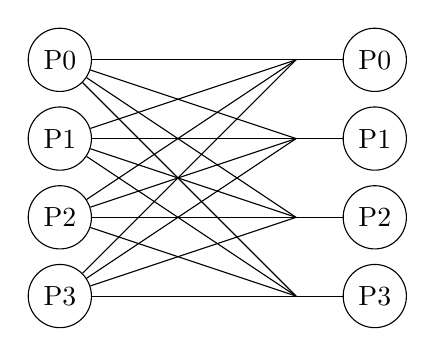
\begin{tikzpicture}
    % Nodos
    \node[draw, circle] (A) at (0,3) {P0};
    \node[draw, circle] (B) at (0,2) {P1};
    \node[draw, circle] (C) at (0,1) {P2};
    \node[draw, circle] (D) at (0,0) {P3};
    \node[draw, circle] (E) at (4,3) {P0};
    \node[draw, circle] (F) at (4,2) {P1};
    \node[draw, circle] (G) at (4,1) {P2};
    \node[draw, circle] (H) at (4,0) {P3};

    % Aristas
    \draw (A) -- (3,3);
    \draw (B) -- (3,3);
    \draw (C) -- (3,3);
    \draw (D) -- (3,3);
    \draw (3,3) -- (E);

    \draw (A) -- (3,2);
    \draw (B) -- (3,2);
    \draw (C) -- (3,2);
    \draw (D) -- (3,2);
    \draw (3,2) -- (F);

    \draw (A) -- (3,1);
    \draw (B) -- (3,1);
    \draw (C) -- (3,1);
    \draw (D) -- (3,1);
    \draw (3,1) -- (G);

    \draw (A) -- (3,0);
    \draw (B) -- (3,0);
    \draw (C) -- (3,0);
    \draw (D) -- (3,0);
    \draw (3,0) -- (H);
\end{tikzpicture}
\caption{Todos combinan.}
\label{graph:colectivas1}
\end{figure}

\begin{figure}
\centering
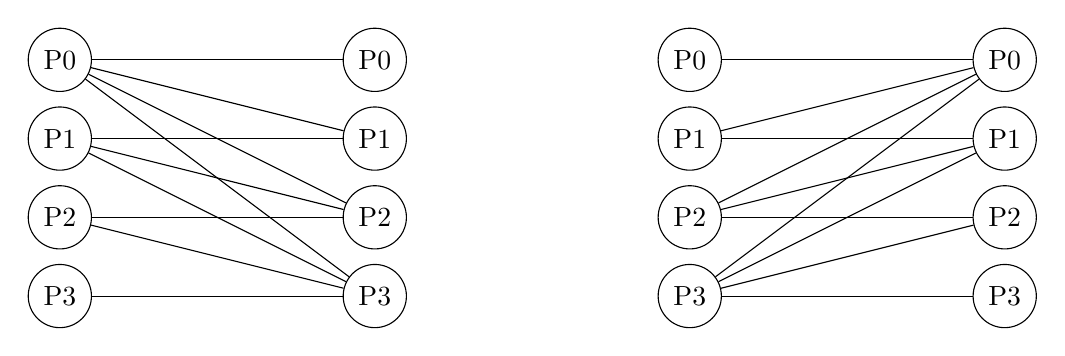
\begin{tikzpicture}
    % Nodos prefijo
    \node[draw, circle] (A) at (0,3) {P0};
    \node[draw, circle] (B) at (0,2) {P1};
    \node[draw, circle] (C) at (0,1) {P2};
    \node[draw, circle] (D) at (0,0) {P3};
    \node[draw, circle] (E) at (4,3) {P0};
    \node[draw, circle] (F) at (4,2) {P1};
    \node[draw, circle] (G) at (4,1) {P2};
    \node[draw, circle] (H) at (4,0) {P3};

    \draw (A) -- (E);
    \draw (A) -- (F);
    \draw (A) -- (G);
    \draw (A) -- (H);
    \draw (B) -- (F);
    \draw (B) -- (G);
    \draw (B) -- (H);
    \draw (C) -- (G);
    \draw (C) -- (H);
    \draw (D) -- (H);

    % Nodos sufijo
    \node[draw, circle] (I) at (8,3) {P0};
    \node[draw, circle] (J) at (8,2) {P1};
    \node[draw, circle] (K) at (8,1) {P2};
    \node[draw, circle] (L) at (8,0) {P3};
    \node[draw, circle] (M) at (12,3) {P0};
    \node[draw, circle] (N) at (12,2) {P1};
    \node[draw, circle] (O) at (12,1) {P2};
    \node[draw, circle] (P) at (12,0) {P3};

    \draw (I) -- (M);
    \draw (J) -- (M);
    \draw (J) -- (N);
    \draw (K) -- (M);
    \draw (K) -- (N);
    \draw (K) -- (O);
    \draw (L) -- (M);
    \draw (L) -- (N);
    \draw (L) -- (O);
    \draw (L) -- (P);
\end{tikzpicture}
\caption{Recorrido en prefijo a la izquierda y recorrido en sufijo a la derecha.}
\label{graph:colectivas2}
\end{figure}

% ----------------------------------------------------------------------

\subsubsection{Implementación en OpenMP} 
Varias comunicaciones de las anteriormente descritas podemos llevarlas a cabo usando la herramienta OpenMP:
\begin{description}
    \item [Uno-a-todos] Podemos llevar a cabo la difusión (lo haremos en la Sesión II de prácticas) con:
        \begin{itemize}
            \item La cláusula \verb|firstprivate| desde el thread 0.
            \item La directiva \verb|single| con la cláusula \verb|copyprivate|. 
            \item La directiva \verb|threadprivate| y uso de la cláusula \verb|copyin| en directiva \verb|parallel| desde thread 0.
        \end{itemize}
    \item [Todos-a-uno] Podemos implementar reducción (lo haremos en la Sesión II de prácticas) con la cláusula \verb|reduction|. 
    \item [Servicios compuestos] En la Sesión I de prácticas hemos usado la directiva \verb|barrier|, que implementa una barrera.
\end{description}
Observemos el trabajo a alto nivel que nos facilitan las diversas directivas propias de una API de directivas y funciones.

\subsubsection{Implementación en MPI} 
Por otra parte, podemos implementar las comunicaciones de una forma más cercana al hardware (a más bajo nivel) con una API de funciones tal y como lo es MPI:
\begin{description}
    \item [Uno-a-uno] De forma asíncrona, con las funciones \verb|MPI_Send()| y \verb|MPI_Receive()|.
    \item [Uno-a-todos] Podemos implementar:
        \begin{itemize}
            \item Difusión, con la función \verb|MPI_Bcast()|.
            \item Dispersión, con la función \verb|MPI_Scatter()|.
        \end{itemize} 
    \item [Todos-a-uno] Como:
        \begin{itemize}
            \item Reducción, con la función \verb|MPI_Reduce()|.
            \item Acumulación, con la función \verb|MPI_Gather()|.
        \end{itemize}
    \item [Todos-a-todos] Podemos implementar ``todos acumulan'' con la función \verb|MPI_Allgather()|.
    \item [Servicios compuestos] Como:
        \begin{itemize}
            \item Todos combinan, con la función \verb|MPI_Allreduce()|.
            \item Barreras, con la función \verb|MPI_Barrier()|.
            \item Scan, con la función \verb|MPI_Scan()|.
        \end{itemize}
\end{description}

\subsection{Paradigmas de programación paralela}
Cada tipo de arquitectura paralela (según la taxonomía de Flynn anteriormente estudiada) presenta distintas implementaciones en cuanto a su diseño se refiere. Es por esto que para cada tipo de arquitectura buscaremos un tipo de código que mejor se adapte a su diseño. Destacamos tres principales paradigmas en cuanto a programación paralela, cada uno asociado a un tipo de arquitectura:
\begin{itemize}
    \item Paso de mensajes (para multicomputadores).
    \item Variables compartidas (para multiprocesadores). 
    \item Paralelismo de datos (para computadores SIMD).
\end{itemize}
Con \emph{paso de mensajes} se supone que cada procesador del sistema tiene su propio espacio de direcciones. Los mensajes llevan datos de un espacio de direcciones a otro y pueden aprovecharse para sincronizar procesos. Los datos transferidos estarán duplicados en el sistema de memoria. Con \emph{variables compartidas}, se supone que los procesasdores comparten espacio de direcciones. Se realiza la transferencia de forma implícita usando instrucciones de lectura y escritura en memoria. Con \emph{paralelismo de datos} la misma instrucción se ejecuta en paralelo en múltiples cores de forma que cada uno actúa sobre un conjunto de datos distinto. Este paradigma es apropiado para aquellas arquitecturas que solo soportan paralelismo a nivel de bucle. La sincronización se encuentra implícita. 

Asimismo, también podemos encontrar herramientas que permiten programar multiprocesadores mediante paso de mensajes, un software que se apoya en el hardware para variables compartidas. De igual forma, hay herramientas que permiten variables compartidas en multicomputadores. Hay lenguajes que soportan paralelismo de datos, tanto en multiprocesadores como en multicomputadores.

\begin{description}
    \item [Paso de mensajes]~\\
        Se dispone de diversas herramientas software, como lenguajes de programación (Ada, Occam, \ldots) o bibliotecas de funciones (como MPI). Los fabricantes de supercomputadores suelen proporcionar este tipo de software, capaz de extraer un gran rendimiento de sus máquinas. Las funciones básicas de comunicación suelen ser \verb|send()| y \verb|receive()|. Generalmente, en la función \verb|send| se especifica el proceso destino y el mensaje a enviar, mientras que en \verb|receive| se especifica la fuente y la estructura de datos en la que se almacenará el mensaje. Podemos encontrar implementaciones \emph{síncronas} (el proceso que ejecuta un \verb|send| se bloquea hasta que el destinatario hace uso de \verb|receive| y viceversa) o \emph{asíncronas} (\verb|send| no tiene por qué bloquear el proceso). Para esta última, es necesario usar un buffer en su implementación. 
    \item [Variables compartidas]~\\
        Encontramos software como lenguajes de programación (Ada 95 o Java), bibliotecas de funciones y APIs de directivas y funciones (como OpenMP). Los propios fabricantes ofrecen compiladores secuenciales con estas extensiones para programar sus máquinas. Para la comunicación se suelen desarrollar instrucciones de \emph{lectura} y \emph{escritura} en memoria, las cuales serán usadas por distintos procesos (en el SO, las hebras comparten memoria entre sí, por lo que no es necesario que usen estas instrucciones). El software ofrece mecanismos para implementar sincronización (para que un proceso no lea antes de que el otro escriba), como cerrojos, semáforos, variables condicionales, \ldots 
        OpenMP dispone además de directivas para llevar a cabo paralelismo de datos (directiva \verb|for|), de tareas (directiva \verb|sections|), y muchas más funcionalidades. 
    \item [Paralelismo de datos]~\\
        En este paradigma se aprovecha el paralelismo de datos inherente a aplicaciones en la que los datos se organizan en estructuras como vectores o matrices. El programador escribe un programa con construcciones que permiten aprovechar paralelismo de datos (como paralelización de bucles, instrucciones vectoriales,~\ldots), así como construcciones para distribuir los datos (la carga de trabajo) entre los núcleos de procesamiento. El programador no lleva a cabo las sincronizaciones (se encuentran implícitas). Ejemplos software son Fortran 95, HPF (High Performance Fortran), NVIDIA CUDA, \ldots
\end{description}

\subsection{Estructuras típicas de códigos paralelos}
Analizando las estructuras (los grafos) de las tareas y de los procesos (junto con las comunicaciones y sincronizaciones entre estos) que componen distintos programas paralelos, se puede encontrar que hay ciertos patrones que se repiten en distintos programas y dentro de un programa. Entre estas estructuras encontramos:
\begin{itemize}
    \item Dueño-esclavo (\emph{master-slave}), o ``granja de tareas'' (\emph{task-farming}).
    \item Cliente-servidor (\emph{client-server}).
    \item Paralelismo de datos, descomposición de datos, o descomposición de dominio. 
    \item Estructura segmentada (\emph{pipeline}), o flujo de datos.
    \item Divide y vencerás (\emph{divide and conquer}), o descomposición recursiva. 
\end{itemize}
Hay estructuras que quizás no se puedan clasificar en un solo tipo de los anteriores. Por otra parte, nos podemos encontrar dentro de un mismo programa paralelo varias de estas estructuras, en distintos niveles.

\subsubsection{Dueño-esclavo} 
En este caso, contamos con un proceso denominado dueño (o \emph{master}) y con varios procesos denominados esclavos (o \emph{slaves}). El dueño se encarga de distribuir las tareas de un conjunto entre el grupo de esclavos, y de ir recolectando los resultados parciales que van calculando los esclavos, con los que el dueño obtiene el resultado final. Usualmente, no hay comunicación entre los esclavos.
Puede implementarse con un único programa si el código de los esclavos no es muy complicado (SPMD), con dos programas, si el código de los esclavos es igual (modo mixto MPMD-SPMD), o con múltiples programas (MPMD).
La repartición de carga puede hacerse de forma estática o dinámica.
Un ejemplo de esto es un programa que tiene que calcular los primos hasta un número $n$, y que hace uso de $r$ esclavos para que cada uno calcule los primos que se encuentran en un vector de tamaño $ \nicefrac{n}{r} $. Combinando el resultado de cada esclavo, obtendremos todos los primos.
\begin{figure}[H]
\centering
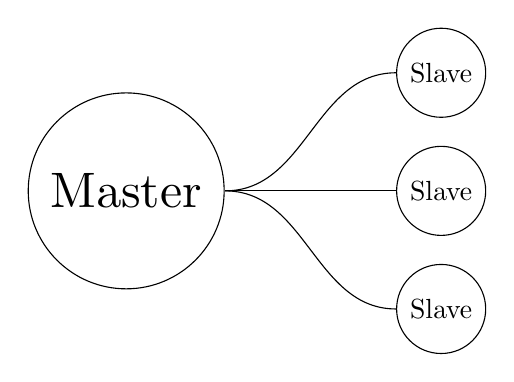
\begin{tikzpicture}
    \node[draw, circle, scale=1.8] (A) at (0,1.5) {Master};
    \node[draw, circle] (B) at (4,0) {Slave};
    \node[draw, circle] (C) at (4,1.5) {Slave};
    \node[draw, circle] (D) at (4,3) {Slave};

    \draw (A) to[out=0,in=180] (B);
    \draw (A) to[out=0,in=180] (C);
    \draw (A) to[out=0,in=180] (D);
\end{tikzpicture}
\caption{Representación gráfica dueño-esclavo.}
\label{graph:dueno_esclavo}
\end{figure}


\subsubsection{Cliente-Servidor} 
También llamado \emph{client-server}, se trata de una estructura similar a dueño-esclavo, pero con los roles invertidos: contamos con múltiples procesos denominados clientes y con un ente (puede ser un proceso, o tener a su vez una estructura paralela distinta en su interior) denominado servidor. En este caso, los clientes son procesos que en un momento determinado solicitan cierta información o servicio al servidor. Este se encarga de procesar la petición y de dar al cliente correspondiente la respuesta esperada. 
Notemos que el servidor puede estar formado a su vez de otras estructuras, como de un sistema dueño-esclavo. Por tanto, podemos tener por un lado a los clientes, que necesitan del servidor un servicio a realizar. Este es el encargado de gestionar los mensajes y de repartir las tareas entre sus esclavos, quienes realizan el cómputo, devolviendo el trabajo realizado al maestro y este a los clientes. 
\begin{figure}[H]
\centering
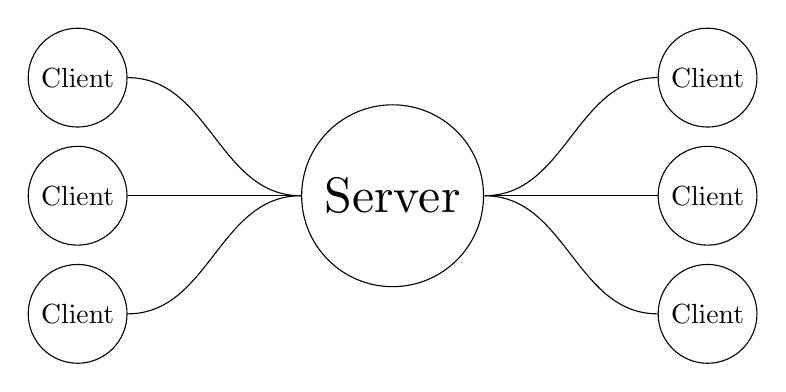
\begin{tikzpicture}
    \node[draw, circle] (E) at (0,0) {Client};
    \node[draw, circle] (F) at (0,1.5) {Client};
    \node[draw, circle] (G) at (0,3) {Client};
    \node[draw, circle, scale=1.8] (A) at (4,1.5) {Server};
    \node[draw, circle] (B) at (8,0) {Client};
    \node[draw, circle] (C) at (8,1.5) {Client};
    \node[draw, circle] (D) at (8,3) {Client};

    \draw (A) to[out=0,in=180] (B);
    \draw (A) to[out=0,in=180] (C);
    \draw (A) to[out=0,in=180] (D);
    \draw (E) to[out=0,in=180] (A);
    \draw (F) to[out=0,in=180] (A);
    \draw (G) to[out=0,in=180] (A);
\end{tikzpicture}
\caption{Representación gráfica cliente-servidor.}
\label{graph:cliente_servidor}
\end{figure}

\subsubsection{Descomposición de datos} 
Alternativa muy utilizada para obtener tareas paralelas en programas con grandes estructuras de datos. La estructura de datos de entrada (o la de salida, o ambas) es dividida en varias partes. A partir de esta división se derivan las tareas paralelas. Estas generalmente realizan operaciones similares. Los algoritmos con imágenes, por ejemplo, admiten una descomposición de datos.
En este esquema, cada proceso puede englobar una o varias tareas. Los diferentes procesos ejecutan normalmente el mismo código (SPMD), que se ejecuta sobre distintos conjuntos de datos. Puede haber comunicaciones entre los distintos procesos.
Un ejemplo de descomposición de datos es el siguiente código, donde se invierten los colores de una imagen de tamaño~$N\times N$:
    \begin{minted}[xleftmargin=1cm]{c++}
#pragma omp parallel for
for(int i = 0; i < N; i++)
    for(int j = 0; j < N; j++){
        imagen[i][j] = 255 - imagen[i][j];
    }
    \end{minted}

\subsubsection{Estructura segmentada o flujo de datos} 
Esta estructura aparece en problemas en los que se aplican funciones a un flujo de datos en secuencia distintas (paralelismo de tareas). La estructura de los procesos y de las tareas es la de un cauce segmentado: cada proceso ejecuta por tanto distinto código. Es un caso típico de un programa MPMD puro. Para que resulte apropiada la estructura segmentada, se debe aplicar el proceso a una secuencia de datos de entrada.
Por ejemplo, podemos tener un decodificador de imágenes JPEG, que aplica a una secuencia de $N\times N$ píxeles (la imagen de entrada) las siguientes funciones: decodificación de entropía, cuantificación inversa, transformada del coseno inversa y conversión RGB\@. Este programa podría implementarse con cuatro procesos en una estructura segmentada.
En este tipo de estructura, la comunicación entre procesos es necesaria, y suele ser unidireccional.
\begin{figure}[H]
\centering
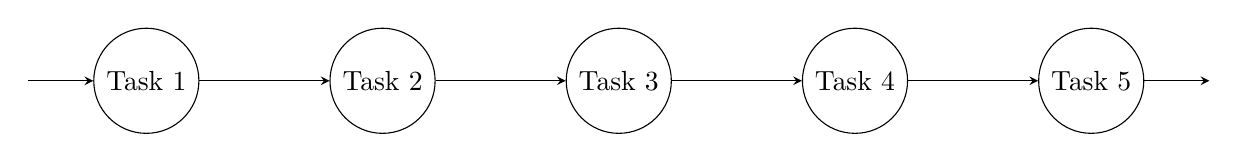
\begin{tikzpicture}
    \node[draw, circle] (A) at (0,0) {Task 1};
    \node[draw, circle] (B) at (3,0) {Task 2};
    \node[draw, circle] (C) at (6,0) {Task 3};
    \node[draw, circle] (D) at (9,0) {Task 4};
    \node[draw, circle] (E) at (12,0) {Task 5};

    \draw[-stealth] (-1.5,0) -- (A);
    \draw[-stealth] (A) -- (B);
    \draw[-stealth] (B) -- (C);
    \draw[-stealth] (C) -- (D);
    \draw[-stealth] (D) -- (E);
    \draw[-stealth] (E) -- (13.5,0);
\end{tikzpicture}
\caption{Representación gráfica de una estructura segmentada.}
\label{graph:estructura_segmentada}
\end{figure}

\subsubsection{Divide y vencerás} 
Se utiliza cuando un problema puede dividirse en dos o más subproblemas de menor tamaño de forma que cada uno pueda resolverse independientemente y combinar al final las distintas soluciones. Si los subproblemas son a su vez instancias más pequeñas del problema original, entonces se podrán volver a subdividir de forma recursiva. Las tareas presentan, por tanto, una estructura de árbol, de forma que no habrá interacciones (comunicaciones o sincronizaciones) entre las tareas que cuelgan del mismo padre.
Un ejemplo de uso de esta estructura podemos verlo cuando nos disponemos a sumar todas las componentes de un vector: podemos dividir el vector en 2, obteniendo dos subproblemas de tamaño $ \nicefrac{n}{2} $, siendo $n$ el número de componentes del vector. Podemos seguir recursivamente dividiendo el vector hasta obtener vectores de tamaño relativamente pequeños, donde haríamos su suma iterativamente. Obtenemos así al final la suma de todas las componentes del vector.

\begin{figure}[H]
\centering
\begin{tikzpicture}
    \node[draw, circle, scale=1.8] (A) at (0,3) {$n$};
    \node[draw, circle, scale=1.3] (B) at (-2,1) {$\nicefrac{n}{2}$};
    \node[draw, circle, scale=1.3] (C) at (2,1) {$\nicefrac{n}{2}$};
    \node[draw, circle, scale=1.3] (D) at (-3,-1) {$\nicefrac{n}{4}$};
    \node[draw, circle, scale=1.3] (E) at (-1,-1) {$\nicefrac{n}{4}$};
    \node[draw, circle, scale=1.3] (F) at (1,-1) {$\nicefrac{n}{4}$};
    \node[draw, circle, scale=1.3] (G) at (3,-1) {$\nicefrac{n}{4}$};

    \draw (A) -- (B);
    \draw (A) -- (C);
    \draw (B) -- (D);
    \draw (B) -- (E);
    \draw (C) -- (F);
    \draw (C) -- (G);
\end{tikzpicture}
\caption{Representación gráfica de divide y vencerás.}
\label{graph:dyv}
\end{figure}


\newpage
\section{Proceso de paralelización}
Cuando queremos obtener una versión paralela de una aplicación con una biblioteca de funciones con directivas o con un lenguaje de programación paralelo, pueden seguirse los siguientes pasos:
\begin{itemize}
    \item Descomposición de la aplicación en tareas independientes.
    \item Asignación de las tareas a procesos o hebras. 
    \item Redactar el código paralelo. 
    \item Evaluación de los tres pasos anteriores.
\end{itemize}
Estudiaremos a lo largo de esta sección todos estos pasos a fondo, junto con un ejemplo práctico.

\subsection{Objetivos}
Esta sección está dedicada a:
\begin{itemize}
    \item Programar en paralelo una aplicación sencilla.
    \item Distinguir entre asignación estática y dinámica, destacando sus ventajas e inconvenientes.
\end{itemize}

\subsection{Descomposición en tareas} 
En esta etapa, tenemos que buscar unidades de trabajo en la aplicación que puedan ejecutarse en paralelo (es decir, que sean independientes). Estas unidades, junto con los datos que usan, forman las \emph{tareas}. Es conveniente en este paso representar las tareas y las relaciones entre ellas mediante un grafo, para observar las dependencias entre estas y el nivel de paralelización de la aplicación. Podemos situarnos en dos niveles de abstracción:
\begin{description}
    \item [Nivel de función] Analizando las dependencias entre las funciones del código podemos encontrar aquellas que son independientes (o aquellas que pueden hacerse independientes), que serán las que se ejecutarán en paralelo. Estamos extrayendo paralelismo de tareas en nuestra aplicación.
    \item [Nivel de bucle] Analizando las iteraciones de los bucles dentro de una función, podemos encontrar si son (o se pueden hacer) independientes. Podemos así detectar paralelismo de datos. Además, si una función consta de varios bucles, puede verse la relación entre estos, para así ver si pueden ejecutarse en paralelo.
\end{description}

\subsubsection{Ejemplo} 
Para paralelizar el cálculo de $\pi$, puede partirse de una versión secuencial disponible o de un planteamiento para el problema que se preste a paralelización. Procedemos pues a realizar este según el segundo método:

Podemos definir el cálculo de $\pi$ como un problema de integración, susceptible de ser paralelizado. Podemos calcular la integral definida en el intervalo $[0,1]$ de la derivada de la arcotangente de $x$:
\begin{equation*}
    \left.\begin{array}{rcl}
        \text{arctg}'(x) & = & \dfrac{1}{1+x^2} \\
                  & & \\
        \text{arctg}(1) & = & \nicefrac{\pi}{4} \\
        \text{arctg}(0) & = & 0 
    \end{array}\right\} \Longrightarrow \int_{0}^{1} \dfrac{dx}{1+x^2} = [\text{arctg}(x)]_0^1 = \dfrac{\pi}{4} - 0
\end{equation*}
Y así multiplicar por 4 para obtener $\pi$. Esta integral puede obtenerse mediante métodos de integración numérica (rectángulo izquierdo, rectángulo derecho, punto medio, trapecio, fórmula de \emph{Simpson}, \ldots). Podemos dividir el área de la derivada del arcotangente en $[0,1]$ en subintervalos, calculando el área de la función en cada subintervalo y sumando. Cuantos más subintervalos tengamos, más exacta será la aproximción.
Notemos que el cálculo del área de los diferentes intervalos es independiente, por lo que podemos repartir estos cálculos en un conjunto de procesadores. Si se divide el intervalo en 100 subintervalos y tenemos 10 procesadores, podemos asignar a cada procesador el cálculo de 10 subintervalos. Sobre código, tenemos lo siguiente:
    \begin{minted}[xleftmargin=1cm]{c++}
main(int argc, char** argv){
    double ancho, x, sum = 0;
    int intervalos;

    intervalos = atoi(argv[1]);
    ancho = 1.0 / (double) intervalos;

    for(int i = 0; i < intervalos; i++){
        x = (i + 0.5) * ancho;
        sum += 4.0 / (1.0 + x*x);
    }

    sum *= ancho;
}
    \end{minted}
Para su paralelización, tratamos de determinar si las iteraciones del bucle son independientes. Como podemos ver, entre las iteraciones existen dependencias, ya que se escribe y se lee en la misma variable \verb|sum|. Sin embargo, estas dependencias pueden eliminarse fácilmente: basta suponer que cada iteración distinta escribe en una variable que depende de \verb|i|. La suma de todas estas variables dará la aproximación de $\pi$. 

\subsection{Asignación de tareas} 
En esta etapa, tratamos de realizar la asignación de las tareas del grafo de dependencias a procesos y a hebras. Por lo general, no es conveniente asignar más de un proceso o hebra por procesador dentro de una misma aplicación (para que no compitan entre ellos). Por tanto, la asignación a procesos o hebras está ligada a la asignación en procesadores. Podemos incluso realizar asignaciones de procesos a procesadores. 

La granularidad de los procesos y las hebras depende del número de procesadores: cuanto mayor sea, menos tareas se asignarán a cada proceso (o hebra). Además, la granularidad depende del tiempo de comunicación y sincronización, debido a que el tiempo de ejecución en paralelo no solo depende del código en sí mismo, sino de las comunicaciones y sincronizaciones entre procesos. Para disminuir este tiempo, pueden asignarse más tareas a un proceso (o hebra), reduciendo así el número de interacciones (comunicaciones o sincronizaciones) entre las tareas a través de la red de comunicación. 

La posibilidad de usar procesos o hebras depende de varios factores:
\begin{itemize}
    \item La arquitectura en la que se va a ejecutar: en un SMP y en procesadores multihebra es más eficiente usar hebras\footnote{Como bien ya sabemos gracias a Sistemas Operativos.}. En arquitecturas mixtas (como clúster de SMP), sería conveniente usar tanto hebras como procesos, especialmente si el número de procesadores en un SMP es mayor que el número de nodos en un cúster.
    \item El sistema operativo debe ser multihebra para poder utilizar hebras (a no ser que las emulemos mediante una biblioteca de hebras, lo que introduce un costo adicional).
    \item Para usar hebras (también para procesos), las herramientas de programación que utilicemos deben permitir poder crearlas.
\end{itemize}
Como regla general, se tiende a asignar las iteraciones de un bucle (paralelismo de datos) a hebras y las funciones (paralelismo de tareas) a procesos.

\subsubsection{Tener en cuenta la arquictura}
La asignación debería repartir la carga de trabajo (el tiempo de cálculo), optimizando la comunicación y la sincronización entre las tareas (minimizándolas), de forma que todos los procesadores empiecen y terminen a la vez (idealmente). En el grafo de tareas previamente mencionado, veíamos tiempos de ejecución aproximados (sabiendo qué trabajo le estamos dando a qué tarea) y sincronizaciones entre estas (visualizando los arcos entre los nodos). Para realizar la asignación cumpliendo todo esto, conviene tener clara la arquitectura (prestaciones de los nodos de ejecución y de la red de comunicación).

Por un lado, la arquitectura puede ser \textbf{heterogénea} u \textbf{homogénea}. Si es heterogénea, consta de componentes con diferentes prestaciones. Por tanto, una buena repartición de carga de trabajo es asignar a los nodos de cómputo más rápido las tareas más pesadas. 

Una arquitectura homogénea (aquella donde los nodos de cómputo son iguales, o casi) puede ser a su vez \textbf{uniforme} o \textbf{no uniforme} (decimos que las arquitecturas uniformes y no uniformes están dentro de las homogéneas porque las heterogéneas son normalmente no uniformes, luego no merece la pena concretar esos casos):
\begin{description}
    \item [Uniforme]~\\
        Si es uniforme, la comunicación de los procesadores con memoria (y probablemente con otros componentes, como E/S) supone el mismo tiempo sean cuales sean los dos componentes que intervienen. Las arquitecturas homogéneas uniformes son en las que menos tenemos que tener en cuenta la arquitectura para la asignación de tareas. Sin embargo, hay arquitecturas homogéneas uniformes en las que una buena asignación puede disminuir el número de colisiones en el acceso a la red.
    \item [No uniforme]~\\
        Si es no uniforme, la velocidad de comunicación entre procesadores con memoria (y probablemente con otros componentes) depende del procesador que queramos que acceda a qué posición de memoria. En este tipo de arquitecturas es más difícil asignar las tareas (código y datos) de forma que se minimice el tiempo de comunicación y sincronización y, en general, el tiempo de ejecución. Pueden eliminarse comunicaciones asignando varias tareas al mismo procesador. 
\end{description}

\subsubsection{Asignar tareas a procesadores}
La asignación de tareas (procesos o hebras) a procesadores puede realizarse de forma \textbf{estática} (en tiempo de compilación o al escribir el programa) o \textbf{dinámica} (en tiempo de ejecución). La asignación dinámica es útil para evitar repartos complejos de tareas en sistemas heterogéneos, especialmente cuando no se conoce el número total de tareas que se van a ejecutar antes de la ejecución. Además, permite que la aplicación se ejecute exitosamente si algún procesador falla. Sin embargo, esta asignación consume un tiempo adicional de sincronización y comunicación.

Un ejemplo de asignación estática es asignar iteraciones consecutivas de un mismo bucle a procesos consecutivos (\textit{round-robin}), mientras que también podemos asignar iteraciones consecutivas a un mismo proceso (continua), como es el caso del bucle \verb|for| en OpenMP\@ (en su asignación por defecto). Un ejemplo de asignación dinámica es almacenar en una variable el índice de la siguiente iteración a ejecutar, de forma que el primer procesador desocupado lea el índice que le indique qué iteración ejecutar, aumentando su valor para que el siguiente procesador desocupado realice la siguiente. Notemos que este acceso a una variable que indique la siguiente iteración debe realizarse en exclusión mutua (por ejemplo, usando un cerrojo). Con paso de mensajes, la asignación dinámica podría hacerse desde el proceso dueño en un sistema dueño-esclavo. Hay herramientas como OpenMP que permiten que el procesador deje al compilador la asignación de tareas a procesos (o hebras).

\begin{ejemplo}
    Si retomamos el ejemplo de la sección anterior en un sistema (por ejemplo) homogéneo uniforme, nos gustaría que la carga de trabajo se distribuya por igual en todos los procesadores. Por tanto, nos interesa más usar una asignación estática frente a una dinámica, debido a que esta última perjudicarían considerablemente las prestaciones debido a la comunicación adicional que añaden.
\end{ejemplo}
\subsection{Código paralelo}
El código que queremos desarrollar va a depender del estilo de programación que se utilice (variables compartidas, paso de mensajes, paralelismo de datos), del modo de programación (SPMD, MPMD, mixto), del punto de partida (versión secuencial, descripción del problema), de la herramienta software que usemos (lenguajes de programación, compiladores, bibliotecas de funciones, APIs de funciones y directivas,~\ldots) y de la estructura (granja de tareas, segmentada, descomposición de datos, divide y vencerás, maestro-esclavo, \ldots) elegida. Todas estas a su vez dependen de la aplicación que queremos paralelizar.
Habrá que añadir o utilizar en el programa las funciones, directivas o construcciones del lenguaje que hagan falta para:
\begin{enumerate}
    \item Crear y terminar procesos (o hebras).
    \item Localizar paralelismo.
    \item Asignar la carga de trabajo conforme a las decisiones tomadas.
    \item Comunicar y sincronizar las diferentes tareas (procesos o hebras).
\end{enumerate}

\subsubsection{Ejemplo implementado con OpenMP}
Hemos decidido implementar el ejemplo que venimos realizando a lo largo de esta sección mediante el estilo de variables compartidas, gracias al modelo que ofrece OpenMP con directivas. Podemos programar con OpenMP a un mayor nivel de abstracción usando directivas (y dejando al compilador que implemente lo que le transmitimos), así como a un menor nivel usando las funciones que nos provee la librería \verb|omp.h| de OpenMP. 

Para obtener el programa paralelo a partir del secuencial ya realizado, hemos añadido a este directivas y funciones necesarias para crear y terminar hebras, asignar tareas a procesos y localizar paralelismo; y comunicar y sincronizar tareas.
\begin{minted}[linenos, xleftmargin=1cm]{c++}
#include <omp.h>
#define NUM_THREADS 4
main(int argc, char** argv){
    double ancho, x, sum = 0;
    int intervalos, i;
    intervalos = atoi(argv[1]);
    ancho = 1.0 / (double) intervalos;

    omp_set_num_threads(NUM_THREADS)
    #pragma omp parallel
    {
        #pragma omp for reduction(+:sum) private(x) schedule(dynamic)
        for(int i = 0; i < intervalos; i++){
            x = (i + 0.5) * ancho;
            sum += 4.0 / (1.0 + x*x);
        }
    }
    sum *= ancho;
}
\end{minted}

\begin{description}
    \item [Crear y terminar hebras] En el programa OpenMP se incluyen funciones que permiten la creación dinámica del grupo de hebras que van a intervenir en el cálculo y que permiten fijar el número de hebras que se crean:
        \begin{itemize}
            \item \verb|omp_set_num_threads()| es una función OpenMP que modifica en tiempo de ejecución el número de hebras que se pueden utilizar en paralelo. Para ello, se sobrescribe el contenido de la variable \verb|OMP_NUM_THREADS|, que contiene dicho número.
            \item \verb|#pragma omp parallel| es una directiva OpenMP que crea un conjunto de hebras. El número será el que tenga la variable \verb|OMP_NUM_THREADS| menos uno, ya que también interviene la hebra \verb|master| en el cálculo. El código de las hebras creadas es el que sigue a esta directiva, que puede ser una o varias sentencias.
        \end{itemize}
    \item [Asignar tareas a procesos y localizar paralelismo] El programador ha dejado el trabajo de repartir las tareas al compilador, simplemente le ha especificado una distribución dinámica, mediante la cláusula \verb|schedule(dynamic)|.
        \begin{itemize}
            \item \verb|#pragma omp for| es una directiva que identifica un conjunto de trabajo compartido iterativo paralelizable y especifica que se distribuyan las iteraciones del bucle \verb|for| entre las hebras del grupo cuya creación se ha especificado con una directiva \verb|parallel|. La política de distribución de las iteraciones del bucle puede especificarse a la directiva mediante la cláusula \verb|schedule(kind[, chunk_size]);|, donde el tipo de distribución puede ser \verb|static, dynamic, runtime| o \verb|guided| (todo esto se verá en el bloque práctico 3).

            \item La cláusula \verb|private(x)| hace que cada hebra tenga una copia privada de la variable \verb|x|. Es decir, no será una variable compartida. La cláusula \verb|reduction(+:sum)| hace que cada hebra utilice una variable local \verb|sum| y que una vez terminada la ejecución de todas las hebras, se sumen todas las variables locales \verb|sum|, almacenando el resultado en una variable compartida \verb|sum|. La directiva \verb|for| obliga a que todas las hebras se sincronicen al terminar el bucle (a no ser que se especifique \verb|nowait|).
        \end{itemize}
        Usando esta directiva \verb|for| se libera trabajo al programador, al no tener que implementar la distribución dinámica ni comunicaciones y sincronizaciones para obtener la suma total (así como las declaraciones de las variable locales \verb|sum|). Además, incluye una barrera implícita que tampoco tiene que incluir el programador. La asignación de hebras a procesadores la hará el sistema operativo, aunque para incrementar las prestaciones, el programador puede orientarlo sobre dicha asignación.
    \item [Comunicación y sincronización] 
        Como ya se ha mencionado, se distribuyen las iteraciones del bucle entre hebras de forma dinámica, de forma que cada una cuenta con su variable local \verb|sum| que resulta en una variable compartida \verb|sum| que al final contiene a la suma de todas las variables locales (todo esto gracias a la cláusula \verb|reduction(+:sum)|). Se está utilizando una comunicación colectiva. Además, se usa una barrera implícita tras la finalización de la región afectada por \verb|for| y tras la finalización de la región afectada por \verb|parallel|.
\end{description}

\subsection{Evaluación de prestaciones}
Una vez redactado el programa paralelo, se pueden evaluar sus prestaciones. Si las prestaciones alcanzadas no son las que se requieren, se debe volver a etapas anteriores del proceso de planteamiento y programación. Probablemente se retrocederá más en la abstracción realizada cuando mayor queramos que sea la mejora a realizar. Podemos también elegir otra herramienta de programación que más se adecúe a conseguir la aplicación a desarrollar. Además, no todas estas herramientas ofrecen las mismas prestaciones: depende de su nivel de aprovechamiento de la arquitectura (a menor nivel de abstracción estas sean, mayor será su eficacia).

\newpage
\section{Evaluación de prestaciones}
En la sección del capítulo anterior de evaluación de prestaciones vimos cómo evaluar mejoras realizadas en programas secuenciales. Nos toca ahora evaluar programas paralelos para comprobar si hemos conseguido alcanzar las prestaciones mínimas que requiere la aplicación programada gracias a la paralelización. En programacion paralela, se usa para evaluar las prestaciones de un código paralelo su tiempo de respuesta (\verb|elapsed time| o tiempo de ejecución) y, adicionalmente, su escalabilidad y eficiencia.

\subsection{Objetivos}
Siguiendo con la evaluación en prestaciones de los computadores con aplicaciones paralelas, en esta sección aprenderemos a:
\begin{itemize}
    \item Obtener ganancia y escalabilidad en el contexto de procesamiento paralelo.
    \item Aplicar la Ley de Amdahl en el contexto de procesamiento paralelo.
    \item Comparar la Ley de Amdahl y la ganancia escalable.
\end{itemize}

\subsection{Ganancia en velocidad}
La ganancia en velocidad ($S$) se utiliza para estudiar en qué medida se incrementan las prestaciones al ejecutar una aplicación en paralelo en un sistema con múltiples procesadores frente a un sistema uniprocesador. Este estudio puede interesarnos tanto por evaluar el computador paralelo como por evaluar la implementación paralela de la aplicación.

La ganancia en prestaciones (o ganancia de velocidad, \emph{speedup}) con $p$ procesadores alcanzada al aplicar paralelismo puede obtenerse como:
\begin{equation*}
    S(p) = \dfrac{\text{Prestaciones}(p)}{\text{Prestaciones}(1)}
\end{equation*}

Es decir, dividiendo las prestaciones en un sistema con $p$ procesadores frente a uno uniprocesador ($p=1$). Puesto que las prestaciones son inversas al tiempo de respuesta, obtenemos la siguiente fórmula (que es la que nos va a interesar):
\begin{equation}
    S(p) = \dfrac{T_S}{T_P(p)}\qquad \text{con\ }\qquad  T_P(p) = T_C(p) + T_O(p)
\end{equation}
donde $T_S$ sería el tiempo de ejecución del programa secuencial y $T_P(p)$ el tiempo de ejecución del programa paralelo con $p$ procesadores. Para obtener $T_S$, se debería escoger el mejor programa secuencial que resuelva la aplicación (para solo centrarnos en el cambio de la implementación del paralelismo).

El tiempo de ejecución en paralelo no solo depende del tiempo de cómputo (de cálculo) en paralelo de las tareas detectadas en la aplicación ($T_C(p)$), sino también de un tiempo de penalización o sobrecarga (\emph{overhead}) $T_O(p)$. Este tiempo de sobrecarga es debido a:
\begin{itemize}
    \item El tiempo dedicado a comunicación y sincronización entre procesos.
    \item El tiempo para crear y terminar los procesos y hebras que permiten la paralelización.
    \item El tiempo de ejecución de operaciones añadidas en la versión paralela que no son necesarias en la secuencial.
\end{itemize}
Además, el tiempo de penalización resultante de un mal reparto de carga de trabajo en procesadores también puede incluirse en este $T_O(p)$.
Tanto este tiempo como el tiempo de cómputo dependen del número de procesadores: cuanto mayor sea este, mayor será el grado de paralelismo (número máximo de tareas independientes que pueden ejecutarse en paralelo) de la aplicación aprovechado. A mayor número de procesos involucrados (debido probablemente a un mayor número de procesadores), mayor será el tiempo de sobrecarga\footnote{Si esto no queda claro, observar la enumeración superior.}.

\begin{ejemplo}
    Por ejemplo, disponemos del siguiente código, un bucle de 16 iteraciones donde cada iteración del bucle tiene un tiempo medio de 1 segundo:
    \begin{minted}[xleftmargin=1cm]{c++}
for(int i = 0; i < 16; i++){
    v[i] = f(i);
}
    \end{minted}
    Las iteraciones no están relacionadas entre sí, luego decidimos paralelizar el bucle. Disponemos de 4 procesadores y decidimos dividir el bucle de forma que cada procesador ejecute 4 iteraciones. Tenemos por tanto, unos tiempos:
    \begin{gather*}
        T_S = \unit[60]{s} \\
        T_C(4) = \nicefrac{16}{4} = \unit[4]{s}
    \end{gather*}
    Cabe destacar que tenemos $T_C(4)=\unit[4]{s}$ y no $T_P(4)=\unit[4]{s}$, ya que los costos de creación, comunicación, sincronización, borrado (y probablemente más acciones) de procesos (o hebras) se encuentran presentes. Por tanto, como esperamos un $T_O(4) > 0$, tenemos que $T_P(4) > 4$.
\end{ejemplo}

En el ejemplo anterior, cada iteración del bucle tardaba 1 segundo que, en comparación con los tiempos actuales de creación, comunicación, etc. de procesos (o hebras) es ridículamente grande. Por tanto, podemos esperar un $T_P(4) \approx T_C(4)$. Sin embargo, si cada iteración del bucle tardase 1 milisegundo en vez de 1 segundo, ya sí tendríamos que probablemente el tiempo de ejecución tendría una diferencia relativa mayor con el tiempo de cálculo.

\subsubsection{Escalabilidad}
La representación de la ganancia en función del número de procesadores ($p$) nos permite evaluar la escalabilidad de una implementación o arquitectura paralela. Idealmente, esperaríamos conseguir un tiempo de ejecución paralelo de ${T_P(p) = \nicefrac{T_S}{p}}$ (como se vio en el ejemplo anterior). Para lograrlo, se debería poder \underline{distribuir} todo el programa secuencial en \underline{partes iguales} entre los procesadores, y el tiempo de \underline{sobrecarga} debería ser \underline{despreciable}. En este caso, la ganancia sería:
\begin{equation*}
    S(p) = \dfrac{T_S}{T_P(p)} = \dfrac{T_S}{\nicefrac{T_S}{p}} = p
\end{equation*}
de forma que la escalabilidad sería \emph{lineal}. Para que siempre pueda ser $p$ la ganancia independientemente del valor de $p$, el \underline{grado de paralelismo} debe ser \underline{ilimitado}; es decir, siempre debemos poder dividir el código entre los $p$ procesadores posibles sea cual sea $p$. Debido a estas tres limitaciones, nos planteamos estudiar qué posibilidades se pueden plantear.
Podemos encontrarnos con \emph{escalabilidades superlineales}, casos donde $S(p)>p$ (no son de relevancia ahora mismo). Dos ejemplos de este suceso pueden ser:\label{ej:superlineal}
\begin{itemize}
    \item Estamos trabajando con una estructura de datos grande (como por ejemplo, un vector muy largo) y puede que al repartir el trabajo, reducimos los fallos de caché (un único procesador debería cargar en cada momento un subvector del vector con el que trabajamos. Sin embargo, puede darse que al repartir el vector entre los procesadores, se disminuya su tamaño y se den menos fallos en cada procesador).
    \item Por ejemplo, al realizar una búsqueda lineal sobre un vector, puede que el elemento a buscar se encuentre en la posición $\frac{n}{2}+1$. Si paralelizamos el código de forma que una hebra busque en las primeras $\nicefrac{n}{2}$ posiciones y el segundo en las $\nicefrac{n}{2}$ restantes, la segunda hebra encontrará el elemento deseado en la primera iteración, reduciendo considerablemente el tiempo de ejecución en comparación con la implementación totalmente secuencial del mismo código.
\end{itemize}
Además, hemos considerado que todo el programa secuencial se puede paralelizar, pero en la práctica podemos encontrarnos (de forma bastante frecuente) tareas que no se puedan ejecutar en paralelo y que suponen un tiempo no despreciable. Más aún, no hemos considerado ninguna limitación en el grado de paralelismo, que sí estará limitado en la práctica (por ejemplo, un bucle de $n$ iteraciones tiene un grado de paralelismo de, a lo sumo, $n$). Finalmente, tampoco hemos considerado tiempos de sobrecarga.

Generalizando lo ya visto, impondremos como mínimo que la carga paralelizable pueda repartirse por igual entre los procesadores disponibles (para simplificar), y además que el tiempo de ejecución $T_S$ es constante (aún variando el número de procesadores). Con estas restricciones generales, procedemos a estudiar casos concretos donde ya damos cierta libertad al problema, con la finalidad de estudiar la escalabilidad de cada sistema:
\begin{enumerate}
    \item Comenzamos suponiendo que la fracción no paralelizable del código secuencial es despreciable, que tenemos un grado de paralelismo ilimitado y un tiempo de sobrecarga despreciable. Estamos en el caso inicialmente estudiado como motivación de esta sección, el caso de \textbf{escalabilidad lineal} (o ganancia lineal):
        \begin{equation*}
            S(p) = \dfrac{T_S}{T_P(p)} = \dfrac{T_S}{\nicefrac{T_S}{p}} = p
        \end{equation*}
    \item Ahora, suponemos la presencia de una fracción no despreciable del código secuencial que no puede ser paralelizada. A esta fracción la llamaremos $f$. Además, consideramos al igual que en el punto anterior un grado de paralelismo ilimitado y una sobrecarga despreciable. En este caso tendremos $T_P(p) = T_C(p) = f\cdot T_S + \frac{1-f}{p}\cdot T_S$ debido a que hay una fracción del código secuencial $f$ que no podemos paralelizar y paralelizamos la otra parte, $1-f$, reduciendo el tiempo de forma lineal (al encontrarnos en el caso anterior), obteniendo así una ganancia de:
        \begin{equation*}
            S(p) = \dfrac{1}{f+\dfrac{1-f}{p}}
        \end{equation*}
        Para un cierto número $p$ de procesadores. A medida que aumentamos este número (ya que nos encontramos estudiando la escalabilidad), obtenemos que:
        \begin{equation*}
            \lim_{p\to\infty}S(p) = \dfrac{1}{f}
        \end{equation*}
        Es decir, la escalabilidad de la aplicación paralela se encuentra limitada ($S(p)$ era creciente) por un factor $\nicefrac{1}{f}$, que depende de la fracción de código que no podemos paralelizar (es decir, por mucho que mejoremos la fracción paralelizable, no obtendremos una mejor escalabilidad si no alteramos $f$).
    \item A continuación, nos encontramos en las mismas condiciones que en el punto anterior, con la salvedad de que ya no consideramos un grado ilimitado de paralelismo, sino que será un cierto valor $n$. En este caso, para un $p$ concreto obtendremos la misma ganancia que en el caso anterior:
        \begin{equation*}
            S(p) = \dfrac{1}{f+\dfrac{1-f}{p}}
        \end{equation*}
        Sin embargo, la escalabilidad del modelo estará limitada por:
        \begin{equation*}
            S(n) = \dfrac{1}{f+\dfrac{1-f}{n}}
        \end{equation*}
        Obteniendo un resultado similar al anterior pero en una situación un tanto más realista.
    \item Finalmente, consideraremos el caso en el que tenemos una fracción de código secuencial no paralelizable ($f$), grado de paralelismo ilimitado (para estudiar más fácilmente la escalabilidad) y una sobrecarga no despreciable, que como ya hemos visto, sabemos que aumenta (de forma lineal) conforme lo hace $p$. En este caso, tendremos una ganancia:
        \begin{equation*}
            S(p) = \dfrac{1}{f+\dfrac{1-f}{p}+\dfrac{T_O(p)}{T_S}}
        \end{equation*}
        \begin{proof}
            En primer lugar, calculamos $T_P(p)$:
            \begin{equation*}
                T_P(p) = T_C(p) + T_O(p) = f\cdot T_S + \left(\dfrac{1-f}{p}\right)T_S + T_O(p)
            \end{equation*}
            A continuación, sustituyendo en la fórmula de la ganancia:
            \begin{equation*}
                S(p) = \dfrac{T_S}{T_P(p)} = \dfrac{T_S}{f\cdot T_S + \left(\dfrac{1-f}{p}\right)T_S + T_O(p)} = \dfrac{1}{f+\dfrac{1-f}{p} + \dfrac{T_O(p)}{T_S}}
            \end{equation*}
        \end{proof}
        
        Que con un grado de paralelismo grande obtenemos:
        \begin{equation*}
            \lim_{p\to\infty}S(p) = 0
        \end{equation*}
        Es decir, llega un punto (un grado de paralelismo) a partir del cual si aumentamos el número de procesadores la ganancia deja de crecer y comienza a decrecer. Este decremento se inicia cuando al incrementar $p$ se incrementa el término de la sobrecarga $\nicefrac{T_O(p)}{T_S}$ en mayor medida que se decrementa la parte del cálculo paralelo, de forma que el denominador de la expresión aumenta en lugar de disminuir.
\end{enumerate}

\subsection{Ley de Amdahl}
Como puede deducirse de las ganancias anteriores, estas disminuyen conforme aumenta la fracción de código no paralelizable. Es decir, la mejora en prestaciones depende de la fracción de código no paralelizable. Por lo que la mejora en prestaciones depende de la fracción que no se puede mejorar. Este razonamiento fue formalizado por Gene Amdahl, dando origen a la fórmula:
\begin{equation}
    S(p) \leq \dfrac{p}{1+f(p-1)}
\end{equation}
conocida como la \textbf{Ley de Amdahl}. 
\begin{proof}
    Como ya hemos visto, la intuición de la fórmula proviene de suponer que estamos trabajando en un caso con una fracción de código secuencial no paralelizable $f$ y con una sobrecarga despreciable. Tendremos por tanto que $T_P(p) = T_C(p)$, de forma que una parte de $T_P(p)$ está formada por $f\cdot T_S$ al ser código que no puede paralelizarse y tendremos por otra parte una fracción de $1-f$ código paralelizable con sobrecarga nula, luego con una escalabilidad lineal. Tenemos por tanto que:
    \begin{equation*}
        S(p) = \dfrac{T_S}{T_P(p)} = \dfrac{T_S}{f\cdot T_S+\dfrac{1-f}{p}\cdot T_S} = \dfrac{1}{f+\dfrac{1-f}{p}} = \dfrac{p}{1+f(p-1)}
    \end{equation*}
    Recordemos que habíamos supuesto una sobrecarga nula. Considerando ahora que tenemos una sobrecarga, obtendremos una ganancia en velocidad menor (al ser mayor el denominador de su expresión), luego la ganancia total a la que podemos llegar es la fracción de la Ley de Amdahl, concluyendo así que:
    \begin{equation*}
        S(p) \leq \dfrac{p}{1+f(p-1)}
    \end{equation*}
\end{proof}

La Ley de Amdahl proporciona una visión pesimista de las ventajas de la paralelización, ya que limita la escalabilidad de la aplicación o arquitectura en un factor $\frac{1}{f}$, independientemente del grado de paralelismo y del código que sí puede paralelizarse.\\

Cabe destacar que para conseguir la Ley de Amdahl, hemos supuesto constante el tiempo de ejecución de la aplicación en un sistema uniprocesador, junto con la fracción de código no paralelizable. Sin embargo, en muchas aplicaciones se puede incrementar la fracción de código paralelizable aumentando el tamaño del problema que resuelve la aplicación.

\subsection{Ganancia escalable. Ley de Gustafson}
Los objetivos a la hora de paralelizar una aplicación pueden ser:
\begin{itemize}
    \item Disminuir el tiempo de ejecución hasta uno razonable.
    \item Aumentar el tamaño del problema a resolver, lo que puede llegar (a veces) a incrementar la precisión en el resultado.
\end{itemize}

Por tanto, cuando consigamos el primer objetivo, podemos plantearnos como meta el segundo para mejorar las prestaciones de la aplicación. Supongamos, por tanto, un modelo de código secuencial con una parte no paralelizable y un número $n$ de tareas a paralelizar que puede incrementarse aumentando el tamaño del problema (no confundir $n$ con el tamaño del problema). Considerando despreciable el tiempo de sobrecarga, podemos mantener constante el tiempo de ejecución paralelo $T_P$, variando el número de procesadores $p$ y el número $n$ de forma que $n=k\cdot p$, con $k$ constante. En este caso, el tiempo de ejecución secuencial depende de $n$ ($T_S(n)$). Teniendo en cuenta estas condiciones, la ganancia en prestaciones sería de:
\begin{equation}
    S(p) = \dfrac{T_S(n)}{T_P} = \dfrac{f\cdot T_P + p(1-f)\cdot T_P}{T_P} = p(1-f)+f
\end{equation}
Este valor será consistente si mantenemos constante el tiempo de ejecución en paralelo. En la expresión, el único término variable es $p$. Según la expresión, tenemos que la ganancia depende linealmente del número de procesadores $p$, con una pendiente de $1-f$, que es la fracción de tiempo que supone la ejecución de la parte paralela. Por tanto, cuanto mayor sea $1-f$, mayor será la escalabilidad (al igual que con la Ley de Amdahl, al ser menor $f$). Esta expresión (que mide cuanto escala la estabilidad) se conoce como la Ley de Gustafson.

Mientras que la Ley de Amdahl asume que el tiempo de ejecución secuencial (o tamaño del problema) se mantiene constante y muestra que la ganancia está limitada debido al código no paralelizado (tomando límite cuando $p\to\infty$), Gustafson mantiene constante el tiempo de ejecución paralelo y muestra que la ganancia en función de $p$ puede crecer con pendiente constante. En ambos estudios se desprecia el tiempo de sobrecarga.

\subsection{Eficiencia}
La eficiencia permite evaluar qué tan cerca está la solución a una aplicación con código paralelo (carga de trabajo en general) respecto a la solución que idealmente deberíamos obtener dados los recursos disponibles. Dicho de otra forma, permite evaluar el grado de aprovechamiento de los recursos del sistema. Las prestaciones que se pueden esperar idealmente con $p$ recursos serían las prestaciones que se obtienen con un recurso multiplicado por $p$:
\begin{equation*}
    E(p) = \dfrac{\text{Prestaciones}(p)}{p\cdot \text{Prestaciones}(1)}
\end{equation*}
Teniendo en cuenta la definición de la ganancia, llegamos a que:
\begin{equation}
    E(p) = \dfrac{S(p)}{p}
\end{equation}
Es decir, la eficiencia se obtiene dividiendo la ganancia entre el número de recursos (que es la ganancia ideal). La ganancia máxima es $p$, por lo que la eficiencia máxima es 1. Por otra parte, la ganancia mínima es 1, por lo que la eficiencia mínima será $\nicefrac{1}{p}$.
% Una expresión que refleje en qué medida hay que incrementar el tamaño de los datos para conseguir una eficiencia constante, incluyendo el tiempo de sobrecarga, es una buena forma de evaluar una implementación paralela y/o arquitectura. 


